\chapter[Quadrature]{Numerical Quadrature}

\section{Introduction}

There are many circumstances in mathematical modelling when we need to
evaluate an integral, like
%
\begin{equation}
 \mint{a}{b}{f(x)}{x} .\label{Qua:eq:1}
\end{equation}
%
However, the integrals that can be evaluated analytically are few and
many integrals of great interest in engineering, like, for example,
the error function,
%
\begin{equation}
 \mbox{Erf}(x) = \mint{-\infty}{x}{e^{-\xi^2}}{\xi} \label{Qua:eq:2}
\end{equation}
%
can only be evaluated numerically.

We discuss two major techniques to evaluate integrals
(\textit{quadrature}): the first is based on \textit{interpolation},
the second on \textit{Gaussian quadrature}.

\section{Polynomial interpolation}

If we want to work with any function $f(x)$ numerically we must expect
to represent it using a finite amount of information. Typically this
is done by assuming that we know only the value of the function at a
finite set of points, call \textit{nodes}, $\{x_j\}$, with
$j=0,\ldots,N$. We denote the function values $f_j \equiv f(x_j)$.

One standard approach is to approximate the function $f$ by another
function $g(x)$ which is easy to manipulate and \textit{interpolates}
$f$ at the nodes, i.e.
%
\begin{equation}
  g(x_j) = f_j = f(x_j), \quad j = 0, \ldots, N.
\end{equation}
%
We then use $g$ in place of $f$ wherever necessary, as we shall see
below.

One standard, simple choice of \textit{interpolating function} $g(x)$
is a polynomial. Given the $N+1$ values $f_j$ at the nodes $x_j$ there
is a \emph{unique} polynomial $g$ of order $N$ that interpolates $f$
(as should be clear, as a polynomial of order $N$ has $N+1$
coefficients to be fixed). There are two standard forms of writing
this polynomial explicitly. Here we just show the Lagrange form to
show the explicit construction is possible. Often the Newton form is
used in numerical calculations instead.

First, given the nodes $x_j$, define the \textit{fundamental
  polynomials} $\ell_j(x)$ by
%
\begin{equation}
  \ell_j(x) = \prod_{\substack{i = 0\\i \ne j}}^N \frac{x - x_i}{x_j -
    x_i}, \quad j = 0, 1, \dots, N.
\end{equation}
%
These have the property that $\ell_j(x_j) = 1$ and $\ell_j(x_k) = 0, j
\ne k$. It follows that
%
\begin{equation}
  g(x) = \sum_{j=0}^N f(x_j) \ell_j(x)
\end{equation}
%
is the polynomial of degree $N$ that interpolates the function $f(x)$
at the nodes $x_j$.

In what follows we shall see methods for solving quadrature and
differential equations based on polynomial interpolation. For these
the defining features are the locations of the nodes and the order of
the interpolating polynomial. In many cases the formulas will simplify
greatly from the general Lagrange form above, so each case is treated
separately.

\section[Using polynomial interpolation]{Numerical integration based on polynomial interpolation}

\subsection{Introduction}

We assume that we can evaluate the function at a finite set of points,
called \textit{nodes}, $\{x_j\}$, with $j=0,\ldots, N$ in the interval
$[a,b]$ and we want to estimate~(\ref{Qua:eq:1}).  The idea behind all
the methods based on polynomial interpolation is that we can replace
the function $f(x)$ with a simpler function $g(x)$, i.e.\ a function
whose integral we can evaluate analytically.  We require that the
function $g(x)$ \textit{interpolates} the function $f(x)$, i.e.\ that
it has the same value as $f(x)$ at the nodes:
%
\begin{equation}
  g(x_j) = f(x_j) , \qquad j = 0,1,\ldots,N. \label{Qua:eq:3}
\end{equation}
%
The simplest choice of class of functions $g(x)$ are polynomials and
the different quadrature interpolation methods are differentiated by
the order of the polynomial interpolation.  Formulae based on
polynomial interpolation with equally spaced nodes go under the
generic name of \textit{Newton-Cotes formulae}.

\subsection{Trapezoidal rule}

\begin{figure}
  \centerline{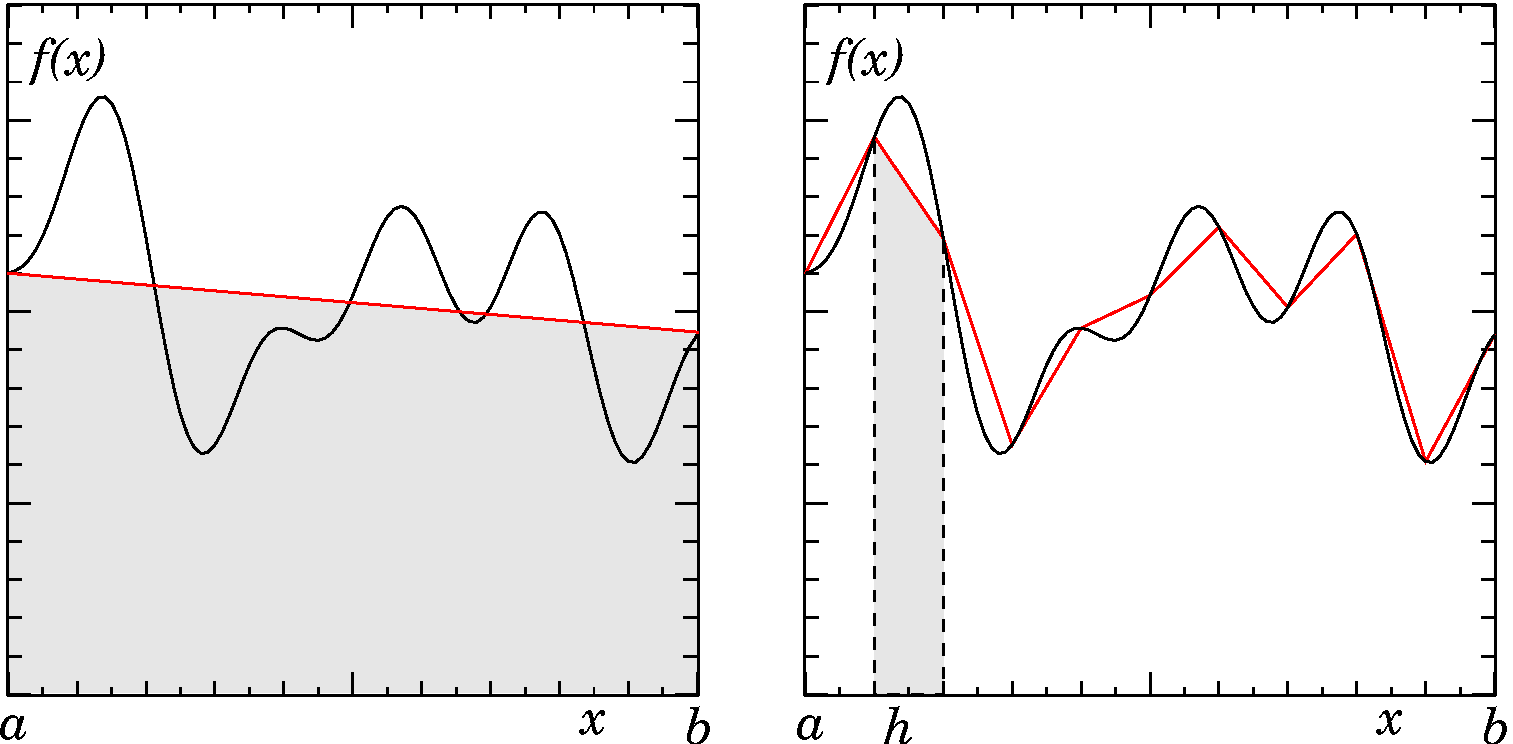
\includegraphics[width=135mm]{figures/trapez}}
  \caption{\label{fig:trapez} \it The trapezoidal rule is based on the
    approximation of the given function $f(x)$ with an order one
    polynomial (left).  In general one uses a composite trapezoidal
    rule: the integration range is divided in intervals of length $h$
    and the function is approximated by a different polynomial on each
    interval (right).}
\end{figure}

The simplest case results if we choose an interpolating polynomial of
order one, i.e.\ we replace the function with a straight line that
interpolates the function at the end points of the integration range
(see left panel of Figure~\ref{fig:trapez}).   The area under the line
is given by
%
\begin{equation}
  A = \frac{1}{2} (b-a) [f(a) + f(b)]
  \label{Qua:eq:32}
\end{equation}
%
and this is the approximate value of~(\ref{Qua:eq:1}) according to the
\textit{trapezoidal rule}.  It is clear that unless the range $[a,b]$
is very small the error in the estimate obtained using the trapezoidal
rule is very large.  The standard procedure is to make use of the
\textit{composite trapezoidal rule}: the integration range is divided
into $N$ intervals of length $h$ and the function $f(x)$ is
approximated on each interval by a straight line that interpolates the
function at the nodes (see right panel of Figure~\ref{fig:trapez}).
The area under each segment of the piecewise linear curve is
%
\begin{equation}
  A_j = \frac{1}{2} (x_{j}-x_{j-1}) [f(x_{j})+f(x_{j-1})] , \quad
  j = 1,2, \ldots, N.
  \label{Qua:eq:4}
\end{equation}
%
By summing all the areas we obtain the composite trapezoidal rule:
%
\begin{equation}
  \mint{a}{b}{f(x)}{x} = \sum_{j=1}^{N} A_j =
  \frac{1}{2} \sum_{j=1}^{N} (x_{j}-x_{j-1}) [f(x_{j})+f(x_{j-1})]
  \label{Qua:eq:5}
\end{equation}
%
If the nodes are equally spaced, i.e.\ if $(x_{j}-x_{j-1}) = h$ for all
$j=1, \ldots, N$, this formula reduces to:
%
\begin{equation}
 \mint{a}{b}{f(x)}{x} =
  \frac{h}{2} \sum_{j=1}^{N} [f(x_{j})+f(x_{j-1})] =
  \frac{h}{2} ( f_0 + 2 f_1 + 2 f_2 + \ldots + 2 f_{N-1} + f_N ) ,
\label{Qua:eq:12}
\end{equation}
%
where $f_j \equiv f(x_j)$.  The error in the approximation is given by
%
\begin{equation}
  \text{Error} \le \frac{1}{12} h^3 N M_2 =
  \frac{(b-a) h^2}{12} M_2 , \qquad
  M_2 = \max_{x\in[a,b]} |f''(x)| .
  \label{Qua:eq:6}
\end{equation}

\subsection{Simpson's rule}

\begin{figure}
  \centerline{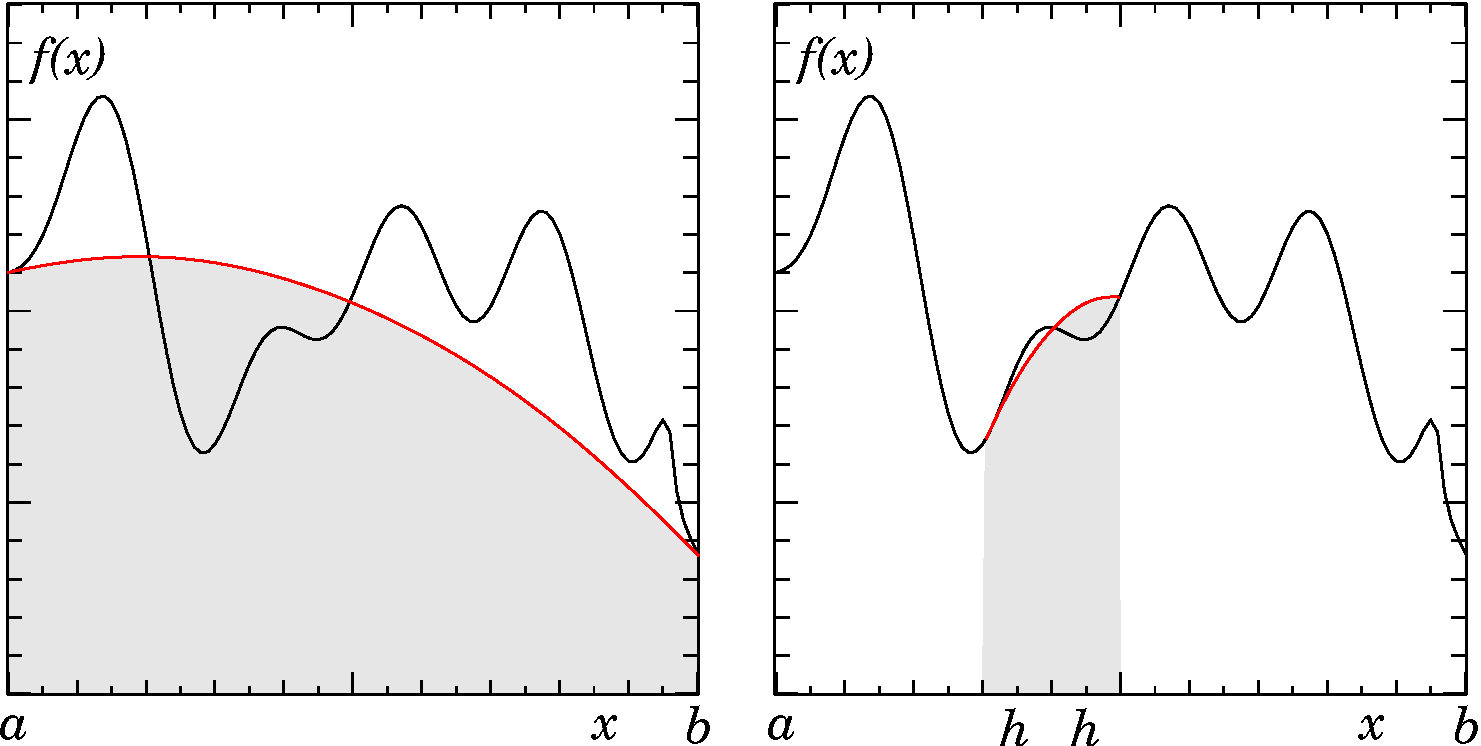
\includegraphics[width=135mm]{figures/simpson}}
  \caption{\label{fig:simpson} \it Simpson's rule is based on the
    approximation of the given function $f(x)$ with an order two
    polynomial (left).  In general one uses a composite Simpson's
    rule: the integration range is divided in intervals of length $2
    h$ and the function is approximated by different parabolas on each
    interval.}
\end{figure}

In this case the function is approximated with a polynomial of order
two (a parabola, see left panel of Figure~\ref{fig:simpson}).  We can
obtain the formula for the quadrature by writing the interpolating
polynomial and integrating it.  It turns out that the area under the
parabola is given by
%
\begin{equation}
  A = \frac{b-a}{6}
  \left [ f(a) + 4 f\left(\frac{a+b}{2}\right) + f(b) \right ],
  \label{Qua:eq:33}
\end{equation}
%
and this is the approximate value of~(\ref{Qua:eq:1}) according to
\textit{Simpson's rule}.  It is clear that unless the range $[a,b]$ is
very small the error in the estimate obtained using the trapezoidal
rule is very large.  The standard procedure is to make use of the
\textit{composite Simpson's rule}: the integration range is divided
into $N/2$ intervals of length $2 h$, with $N$ an even number. The
function $f(x)$ is approximated on each interval by a parabola that
interpolates the function at the nodes (see right panel of
Figure~\ref{fig:simpson}).  For simplicity we assume that the
interpolation points $\{x_j\}$, $j=0,1,2,\ldots,N$ are all equally
spaced so that we can write:
%
\begin{equation*}
  x_j = x_0 + j h .
\end{equation*}
%
The area under the parabola joining the nodes $x_{j-1}$, $x_{j}$ and
$x_{j+1}$ is
%
\begin{equation}
  A_j = \frac{h}{3} \left[f(x_{j-1})+4f(x_{j})+f(x_{j+1})\right]
  \label{Qua:eq:9}
\end{equation}
%
where $j=1,3,5,\ldots, N-1$.  This result is known as
\textit{Simpson's rule}.  If we apply it to all the sub-intervals in
$[a,b]$ we obtain the composite Simpson rule:
%
\begin{equation}
  \mint{a}{b}{f(x)}{x} = \sum_{k=1}^{N/2} A_{2k-1} =
  \frac{h}{3} \left[ f(a) +
    2 \sum_{j=1}^{N/2-1} f(x_{2j}) +
    4 \sum_{j=1}^{N/2} f(x_{2j-1}) + f(b) \right] + R,
  \label{Qua:eq:10}
\end{equation}
%
where the estimate for the error is given by
%
\begin{equation}
  |R|\le \frac{M_4}{180}(b-a)h^4,\label{Qua:eq:11}
\end{equation}
%
where $M_4=\max|f^{(4)}(x)|$ with $a \le x \le b$.  Note that
Simpson's rule is exact for any cubic polynomial as $f^{(4)}(x) \equiv
0$ for all polynomials of order three.

We can obtain an estimate of the error by proceeding as follows.  We
compare the Taylor expansion of Simpson's rule for the integral in the
range $[x_{j-1},x_{j+1}]$, given by equation~(\ref{Qua:eq:9}), to the
Taylor expansion of the exact integral.  The error is the first term
in the difference of the two Taylor expansions.  We start with the
Taylor expansion of the Simpson's rule estimate of
%
\begin{equation}
  \mint{x_{j-1}}{x_{j+1}}{f(x)}{x} \simeq A_j =
  \frac{h}{3} [ f(x_{j-1}) + 4 f(x_{j}) + f(x_{j+1}) ] ,
  \label{Qua:eq:19}
\end{equation}
%
where, to simplify the notation, we use the notation $f_j=f(x_j)$,
$f'_j=f'(x_j)$, and, in general, $f^{(n)}_j$ for the $n$-th derivative
of $f(x)$ evaluated at $x=x_j$.  Using Taylor's theorem to expand
$f(x)$ at $x=x_j$ we can write
%
\begin{equation}
  A_j = 2 h f_j + \frac{h^3}{3} f_j'' + \frac{h^5}{36} f_j^{(4)} + \order{h^6}
  \label{Qua:eq:20}
\end{equation}
%
We now need to compute the Taylor expansion in powers of $h$ of the
exact result.  In order to do this we introduce the function
%
\begin{equation}
  F(t) = \mint{x_j-t}{x_j+t}{f(x)}{x} .
  \label{Qua:eq:21}
\end{equation}
%
Note that with this notation
%
\begin{equation}
  \mint{x_{j-1}}{x_{j+1}}{f(x)}{x} = F(h).
  \label{Qua:eq:14}
\end{equation}
%
Therefore, in order to compute the Taylor expansion in powers of $h$
of the exact result of the integral in equation~(\ref{Qua:eq:14}), we
need to expand $F(t)$ in Taylor series around $t=0$:
%
\begin{equation}
  F(h) = F(0) +
  h \eval{\dv{F}{t}}_{t=0}  +
  \frac{h^2}{2} \, \eval{\dv[2]{F}{t}}_{t=0}  +
  \ldots +
  \frac{h^5}{5!} \, \eval{\dv[5]{F}{t}}_{t=0} +
  \order{h^6}
  \label{Qua:eq:15}
\end{equation}
%
We note that $F(0)=0$.  Moreover, by the fundamental theorem of
calculus (with a little help from the chain rule)
%
\begin{equation*}
  \dv{F}{t} = f(x_j+t) + f(x_j-t) \implies
  \dv[n]{F}{d} = f^{(n-1)}(x_j+t) +
  (-1)^{n+1} f^{(n-1)}(x_j-t) .
\end{equation*}
%
Note that all the even derivatives of $F(t)$ are zero at $t=0$ so that
the Taylor expansion of~(\ref{Qua:eq:15}) becomes
%
\begin{equation}
  2 h f_j + \frac{h^3}{3} f_j'' + \frac{h^5}{60} f_j^{(4)} + \order{h^6}.
  \label{Qua:eq:30}
\end{equation}
%
Combining these two expansions, we have that the local error in the
interval $[x_{j-1},x_{j+1}]$ is, up to order $h^6$,
%
\begin{equation}
  E_j \equiv F(h) - A_j = - \frac{1}{90} h^5 f_j^{(4)} \implies
  \abs{E_j} \le \frac{1}{90} h^5 M_4 ,
  \label{Qua:eq:31}
\end{equation}
%
where $M_4$ is the same as in equation~(\ref{Qua:eq:11}).  Summing the
local errors over all the intervals used in the composite Simpson's
rule gives the total error, $R$,
%
\begin{equation}
  \abs{R} = \abs{\sum_{k=1}^{N/2} E_{2k-1}} \le
  \sum_{k=1}^{N/2} \abs{ E_{2k-1} } \le
  \sum_{k=1}^{N/2} \frac{1}{90} h^5 M_4 = \frac{M_4}{180}(b-a)h^4.
\end{equation}

\subsection{Richardson extrapolation}

This is a very general technique that uses the information on the rate
of decrease of the error to get a better estimate of the numerical
result required.  As such it can be applied to many different
algorithms, not just quadratures.  However, here we illustrate it in
the context of Simpson's rule.

Equation~(\ref{Qua:eq:11}) tells us that the error on the estimate of
the integral decreases with the fourth power of the integration step,
$h$.  However, in order to estimate the error using this formula we
would also need the value of the coefficient $M_4$.  We can get round
this problem by using the following procedure.  Indicate with $I_n$
the estimate of the integral using $n$ intervals and with $I$ the
exact value of the integral.  From~(\ref{Qua:eq:11}) we have that
%
\begin{equation}
  I - I_{2n} \simeq C (2n)^{-4} =
  2^{-4} \left ( C n^{-4} \right ) \simeq 2^{-4} (I - I_n) .
  \label{Qua:eq:16}
\end{equation}
%
In this last step we have assumed that the constant $C$ is the same
whether we use $n$ or $2n$ intervals to estimate the integral.  This
not strictly true, but it is a reasonable approximation if the
integration range is small enough.  From~(\ref{Qua:eq:16}) we have
that the exact value of the integral is approximately
%
\begin{equation*}
  I \simeq \frac{2^4 I_{2 n} - I_n}{2^4 -1}
\end{equation*}
%
and we use this as the new estimate of the integral
(\textit{Richardson extrapolated value}):
%
\begin{equation}
  R_{2 n} = \frac{2^4 I_{2 n} - I_n}{2^4 -1} .
  \label{Qua:eq:22}
\end{equation}
%
The error in the approximation is roughly
%
\begin{equation}
  E_{2n} \equiv \abs{ R_{2 n} - I_{2 n} } = \frac{\abs{I_n - I_{2 n}}}{2^4 -1} .
  \label{Qua:eq:17}
\end{equation}
%
This quantity is called the \textit{computable estimate of the error}.

\subsection{Adaptive quadrature}

Adaptive quadrature methods are intended to compute definite integrals
to a given precision by automatically choosing a set of nodes that
takes into account the behaviour of the integrand by being denser
where the integrand varies more rapidly. Ideally, the user supplies
only the integrand $f$, the interval $[a,b]$, and the accuracy
$\epsilon$ desired for computing the integral
%
\begin{equation}
  \mint{a}{b}{f(x)}{x} . \label{Qua:eq:23}
\end{equation}
%
The program then divides the interval into sub-intervals of varying
length so that numerical integration on these sub-intervals will
produce results of acceptable precision. The main idea is that if
Simpson's rule on a given sub-interval is not sufficiently accurate,
that interval will be divided into two equal parts, and Simpson's rule
will be used on each half. This procedure will be repeated in an
effort to obtain an approximation to the integral with the same
accuracy over all the sub-intervals involved.  A rough algorithm is as
follows:

\begin{enumerate}
  %
\item Compute the integral~(\ref{Qua:eq:23}) using $3$ points and
  estimate the global error.  If the error is smaller than the
  tolerance stop.
  %
\item Divide the interval into two equal parts.  Consider each part in
  turn.
  %
\item Compute the integral on the sub-interval using $3$ points,
  i.e.\ using a finer grid.
%
\item Estimate the error on the evaluation of the integral over the
  sub-interval.  If it is larger than the maximum acceptable local
  error then divide the sub-interval in two and start again from point
  (2).  Otherwise go to point (3) and work on the next sub-interval if
  there are any left.
%
\end{enumerate}

In order to apply this idea we need to firstly to estimate the
\textit{local error}: we can do this using Richardson's extrapolation
and equation~(\ref{Qua:eq:17}).  Secondly, we need to estimate the
\textit{global error} on the integration over the entire interval
$[a,b]$ as a function of the local errors.

\smallskip

\noindent
We indicate with $e_i$ the local error on the integration over the
segment $[x_{i-1},x_i]$. If
%
\begin{equation}
  \abs{e_i} \le \epsilon (x_i-x_{i-1})/(b-a),
  \label{Qua:eq:25}
\end{equation}
%
then the total error will be bounded by
%
\begin{equation}
  \abs{ \sum_{i=1}^n e_i} \le \sum_{i=1}^n \abs{e_i} \le
  \frac{\epsilon}{b-a} \sum_{i=1}^n (x_i-x_{i-1}) = \epsilon.
  \label{Qua:eq:26}
\end{equation}
%
Therefore in the adaptive quadrature algorithm outlined above we have
to ensure that the local error satisfies~(\ref{Qua:eq:25}).

\section{Gaussian Quadrature}

The aim of all quadrature techniques is to create formulae of the type
%
\begin{equation}
  \mint{a}{b}{f(x)}{x} \simeq \sum_{i=1}^n w_i f(x_i) .
 \label{Qua:eq:18}
\end{equation}
%
In the trapezoidal and Simpson's rule the points where the function is
evaluated, $x_i$, are fixed \textit{a priori} and we obtain
that~(\ref{Qua:eq:18}) is exact for all polynomial of degree less than
or equal to $n$.  In the case of the trapezoidal rule we have $n=2$
and the rule is exact for all linear functions.  In the case of
Simpson's rule we have $n=3$ and we would expect the formula to be
exact for all quadratic polynomials.  As a matter of fact, it is exact
for polynomials of order three, but this is due to a happy
cancellation.

However, there is no obligation to fix the nodes.  As a matter of fact
we could fix the coefficients (called \textit{weights}) $w_i$, for
example set them all to one, or we could not fix anything.  The
general criterion to find nodes and weights is to require that
equation~(\ref{Qua:eq:18}) is as accurate as possible, i.e.\ that it is
exact for polynomials of degree as high as possible.  In other words,
we require that the nodes and weights are such that
%
\begin{equation}
  \mint{a}{b}{x^s}{x} = \sum_{i=1}^n w_i x_i^s, \quad s=0,1,...,N,
  \label{Qua:eq:27}
\end{equation}
%
with $N$ as large as possible.

As above, we define the \textit{fundamental polynomials}
$\ell_i(x)$ given by
%
\begin{equation}
  \ell_i(x) = \prod_{\substack{j = 0\\j \ne i}}^N \frac{x - x_j}{x_i -
    x_j}, \quad i = 0, 1, \dots, N,
\end{equation}
%
have the property that $\ell_i(x_i) = 1$ and $\ell_i(x_k) = 0, i \ne
k$. It follows that
%
\begin{equation}
  p(x) = \sum_{i=0}^N f(x_i) \ell_i(x)
\end{equation}
%
is the polynomial of degree $N$ that interpolates the arbitrary
function $f(x)$ at the given nodes $x_i$. If the nodes are known or
fixed we can therefore immediately compute the weights as
%
\begin{equation}
  w_i = \mint{a}{b}{\ell_i(x)}{x}.
\end{equation}
%

If neither the nodes nor the weights are fixed we have $N$ nonlinear
equations for $2n$ unknowns $x_1,...,x_n$ and $w_1,...,w_n$.  One can
show that this problem has a unique solution if $N=2n-1$, i.e.\ that it
is possible to compute exactly the integrals of polynomials of degree
up to $2 n - 1$.  The resulting algorithm is called a {\bf Gaussian
  quadrature}.  There are many formulae for Gaussian quadrature that
depend mainly on the choice of integration interval and on the type of
the integral.  A generic Gauss quadrature formula is
%
\begin{equation}
  \mint{a}{b}{W(x) f(x)}{x} = \sum_{i=1}^n w_i f(x_i)
\end{equation}
%
and the different formulae are summarised in the following table:

\begin{center}
 \begin{tabular}{lll} \hline
  $(a,b)$ & $W(x)$ & Gauss- \\ \hline
  $(-1,1)$ & 1 & Legendre \\
  $(-1,1)$ & $(1-x^2)^{-1/2}$ & Chebychev \\
  $(0,\infty)$ & $x^c e^{-x}$ & Laguerre $c=0,1,\ldots$ \\
  $(-\infty,+\infty)$ & $e^{-x^2}$ & Hermite \\ \hline
 \end{tabular}
\end{center}

\section*{Further reading}

Topics covered here are also covered in
\begin{itemize}
\item Chapter 6 of Linz \& Wang, \textit{Exploring Numerical
    Methods} (QA297 LIN),
\item Chapter 7 of Kincaid \& Cheney, \textit{Numerical Analysis}
  (QA297 KIN),
\item Chapters 7 and 10 of S{\"u}li \& Mayers, \textit{An Introduction
    to Numerical Analysis} (not in library).
\end{itemize}

The issue of representing an arbitrary function by an interpolating
function, which will recur in later chapters, is covered in
considerable detail elsewhere; for example\begin{itemize}
\item Chapters 4 and 5 of Linz \& Wang, \textit{Exploring Numerical
    Methods} (QA297 LIN),
\item Chapter 6 of Kincaid \& Cheney, \textit{Numerical Analysis}
  (QA297 KIN),
\item Chapters 6, 8, 9 and 11 of S{\"u}li \& Mayers, \textit{An Introduction
    to Numerical Analysis} (not in library).
\end{itemize}
